\documentclass[xcolor=pdflatex,dvipsnames,table]{beamer}
\usepackage{epsfig,graphicx}
\usepackage{palatino}
\usepackage{fancybox}
\usepackage{relsize}
\usepackage[procnames]{listings}
\usepackage{hyperref}
\usepackage{qtree} % needed?
\usepackage{booktabs}
\usepackage{dirtree}
\usepackage[normalem]{ulem}


% fatter TT font
\renewcommand*\ttdefault{txtt}
% another TT, suggested by Alex
% \usepackage{inconsolata}
% \usepackage[T1]{fontenc} % needed as well?


\newcommand{\scale}{0.7}

\newcommand{\todo}[1]{{\emph{TODO: #1}}}
\newcommand{\martin}[1]{{\color{blue} Martin: #1}}
\newcommand{\abcdef}[1]{{\color{red} Author2: #1}}

% uncomment following for final submission
%\renewcommand{\todo}[1]{}
%\renewcommand{\martin}[1]{}
%\renewcommand{\author2}[1]{}

\newcommand{\code}[1]{{\texttt{#1}}}

\hypersetup{
  linkcolor  = black,
%  citecolor  = blue,
  urlcolor   = blue,
  colorlinks = true,
}

\beamertemplatenavigationsymbolsempty
\setbeamertemplate{footline}[frame number]





\newif\ifbook
% shared in slides and book

\lstdefinelanguage{chisel}{
  morekeywords={abstract,case,catch,class,def,%
    do,else,extends,false,final,finally,%
    for,if,implicit,import,match,mixin,%
    new,null,object,override,package,%
    private,protected,requires,return,sealed,%
    super,this,throw,trait,true,try,%
    type,val,var,while,with,yield},
  otherkeywords={=>,<-,<\%,<:,>:,\#,@},
  sensitive=true,
  morecomment=[l]{//},
  morecomment=[n]{/*}{*/},
  morestring=[b]",
  morestring=[b]',
  morestring=[b]"""
}

\usepackage{color}
\definecolor{dkgreen}{rgb}{0,0.6,0}
\definecolor{gray}{rgb}{0.5,0.5,0.5}
\definecolor{mauve}{rgb}{0.58,0,0.82}

% Default settings for code listings
\ifbook
\lstset{%frame=lines,
  language=chisel,
  aboveskip=3mm,
  belowskip=3mm,
  showstringspaces=false,
  columns=fixed, % basewidth=\mybasewidth,
  basicstyle={\small\ttfamily},
  numbers=none,
  numberstyle=\footnotesize,
  % identifierstyle=\color{red},
  breaklines=true,
  breakatwhitespace=true,
  procnamekeys={def, val, var, class, trait, object, extends},
  % procnamestyle=\ttfamily,
  tabsize=2,
  float
}
\else
\lstset{%frame=lines,
  language=chisel,
  aboveskip=3mm,
  belowskip=3mm,
  showstringspaces=false,
  columns=fixed, % basewidth=\mybasewidth,
  basicstyle={\small\ttfamily},
  numbers=none,
  numberstyle=\footnotesize\color{gray},
  % identifierstyle=\color{red},
  keywordstyle=\color{blue},
  commentstyle=\color{dkgreen},
  stringstyle=\color{mauve},
  breaklines=true,
  breakatwhitespace=true,
  procnamekeys={def, val, var, class, trait, object, extends},
  procnamestyle=\ttfamily\color{red},
  tabsize=2,
  float
}
\fi

\lstnewenvironment{chisel}[1][]
{\lstset{language=chisel,#1}}
{}

\newcommand{\shortlist}[1]{{\lstinputlisting[nolol]{#1}}}

\newcommand{\longlist}[3]{{\lstinputlisting[float, caption={#2}, label={#3}, frame=tb, captionpos=b]{#1}}}

\newcommand{\verylonglist}[3]{{\lstinputlisting[caption={#2}, label={#3}, frame=tb, captionpos=b]{#1}}}


\title{Communicating State Machines}
\author{Martin Schoeberl}
\date{\today}
\institute{Technical University of Denmark\\
Embedded Systems Engineering}

\begin{document}

\begin{frame}
\titlepage
\end{frame}


\begin{frame}[fragile]{TODO}
\begin{itemize}
\item Repeat stuff
\item Did I do input processing last time? No, do it today
\item Ready/Valid
\item a little bit of Scala
\item add cosimulation to the verification story (show Lipsi), maybe later
\end{itemize}
\end{frame}

\begin{frame}[fragile]{Overview}
\begin{itemize}
\item Repeat
\end{itemize}
\end{frame}

\begin{frame}[fragile]{Last (and Today's) Lab}
\begin{itemize}
\item Display multiplexer
\begin{itemize}
\item Input are 16 switches for 4 hexadecimal digits
\end{itemize}
\item How many have finished it?
\item Please show it a TA when finished for a ``tick''
\item There is a simulation available, show it
\item Maybe extend it with binary to BCD conversion
\begin{itemize}
\item This is optional/advanced material
\end{itemize}
\item You can also start to work on the full Vending Machine
\begin{itemize}
\item Top-level, pin definition, and a simple tester is in:
\item \url{https://github.com/schoeberl/chisel-lab/tree/master/vending}
\end{itemize}
\end{itemize}
\end{frame}


\begin{frame}[fragile]{Next Labs}
\begin{itemize}
\item Next week is Easter break
\item Week after Easter 16/4:
\begin{itemize}
\item 4 hours lab, no lecture
\item Have a short meeting in Zoom to gather
\item Short reminder what the VM is
\item Maybe questions
\end{itemize}
\item Work on the full Vending Machine
\end{itemize}
\end{frame}


\begin{frame}[fragile]{yyy}
\begin{itemize}
\item yyy
\end{itemize}
\end{frame}

\begin{frame}[fragile]{yyy}
\begin{itemize}
\item yyy
\end{itemize}
\end{frame}

\begin{frame}[fragile]{Binary-Coded Decimal (BCD)}
\begin{itemize}
\item Your current display shows numbers in hexadecimal 
\begin{itemize}
\item $15_{10}$ is displayed as $0F_{16}$
\item Which is in binary: 00001111
\item We would like to see it as a `1' followed by a `5'
\item Which is in binary: 0001 0101
\end{itemize}
\item Convert from binary to binary-coded decimal (BCD)
\begin{itemize}
\item But only for the display
\item Computing in BCD is hard
\end{itemize}
\end{itemize}
\end{frame}

\begin{frame}[fragile]{Binary to BCD Conversion Table}
\begin{chisel}
  val bincode = io.sw(7,0)
  val bcd = WireDefault(bincode)

  switch(bincode) {
    is(0.U) { bcd := "b0000_0000".U }
    is(1.U) { bcd := "b0000_0001".U }
    is(2.U) { bcd := "b0000_0010".U }
    // ... some more
    is(9.U) { bcd := "b0000_1001".U }
    is(10.U) { bcd := "b0001_0000".U }
    is(11.U) { bcd := "b0001_0001".U }
    is(12.U) { bcd := "b0001_0010".U }
    // ... and many more entries
  }

  dispMux.io.price := bcd
\end{chisel}
\end{frame}

\begin{frame}[fragile]{Binary-Coded Decimal (BCD)}
\begin{itemize}
\item Conversion is a table (= function)
\item Combinational logic
\item We \emph{could} do the table manually
\begin{itemize}
\item But it is large
\item The table has 100 entries to convert 0 to 99 to BCD
\end{itemize}
\item Let's write a program for this
\item We will write our first \emph{hardware generator}
\item First we need a little bit of Scala
\end{itemize}
\end{frame}



\begin{frame}[fragile]{Chisel and Scala}
\begin{itemize}
\item Chisel is a library written in Scala
\begin{itemize}
\item Import the library with \code{import chisel3.\_}
\end{itemize}
\item Chisel code is Scala code
\item When it is run is \emph{generates} hardware
\begin{itemize}
\item Verilog for synthesize
\item Scala netlist for simulation (testing)
\end{itemize}
\item Chisel is an embedded domain specific language
\item Two languages in one can be a little bit confusing
\end{itemize}
\end{frame}

\begin{frame}[fragile]{Scala}
\begin{itemize}
\item Is object oriented
\item Is functional
\item Strongly typed with very good type inference
\item Runs on the Java virtual machine
\item Can call Java libraries
\item Consider it as Java++
\begin{itemize}
\item Can almost be written like Java
\item With a more lightweight syntax
% \item Scala for Java Refugees is a nice tutorial (but link is dead)
% \item \url{http://www.codecommit.com/blog/scala/roundup-scala-for-java-refugees}
\end{itemize}
\end{itemize}
\end{frame}

\begin{frame}[fragile]{Scala Hello World}
\shortlist{../src/main/scala/HelloScala.scala}
\begin{itemize}
\item Compile with \code{scalac} and run with \code{scala}
\item You can even use Scala as a scripting language
\item Or run with \code{sbt run}
\item Show both
\end{itemize}
\end{frame}

\begin{frame}[fragile]{Scala Values and Variables}
\begin{itemize}
\item Chisel has two type of variables: \code{val}s and \code{var}s
\item A \code{val} cannot be reassigned, it is a constant
\item We use a \code{val} to name a hardware component in Chisel
\end{itemize}
\shortlist{../code/scala_val.txt}
\begin{itemize}
\item Types are usually inferred
\item But can be explicitly stated as follows
\end{itemize}
\shortlist{../code/scala_int_type.txt}
\end{frame}

\begin{frame}[fragile]{Scala Variables}
\begin{itemize}
\item A \code{var} can be reassigned, it is like a classic variable
\item We use a \code{var} to write a hardware generator in Chisel
\end{itemize}
\shortlist{../code/scala_var.txt}
\end{frame}

\begin{frame}[fragile]{Simple Loops}
\shortlist{../code/scala_loop.txt}
\begin{itemize}
\item We use a loop to generate hardware components
\end{itemize}
\end{frame}

\begin{frame}[fragile]{Scala \code{for} Loop for Circuit Generation}
\shortlist{../code/scala_loop_gen.txt}
\begin{itemize}
\item \code{for} is Scala
\item This loop generates several connections
\item The connections are parallel hardware
\item This is a shit register
\end{itemize}
\end{frame}

\begin{frame}[fragile]{Conditions}
\shortlist{../code/scala_condition.txt}
\begin{itemize}
\item Executed at runtime, when the circuit is created
\item This is \emph{not} a mlutplexer
\end{itemize}
\end{frame}

\begin{frame}[fragile]{Scala Arrays and Lists}
\begin{chisel}
// An integer array with 10 elements
val numbers = new Array[Integer](10)
for (i <- 0 until numbers.length) {
  numbers(i) = i*10
}
println(numbers(9))


// List of integers
val list = List(1, 2, 3)
println(list)
// Different form of list construction
val listenum = 'a' :: 'b' :: 'c' :: Nil
println(listenum)
\end{chisel}
\end{frame}


\begin{frame}[fragile]{Scala Classes}
\begin{chisel}
// A simple class
class Example {
  // A field, initialized in the constructor
  var n = 0
  
  // A setter method
  def set(v: Integer) = {
    n = v
  }
  
  // Another method
  def print() = {
    println(n)
  }
}
\end{chisel}
\end{frame}

\begin{frame}[fragile]{Scala (Singleton) Object}
\begin{chisel}
object Example {}
\end{chisel}
\begin{itemize}
\item For \emph{static} fields and methods
\begin{itemize}
\item Scala has no static fields or methods like Java
\end{itemize}
\item Needed for \code{main}
\item Useful for helper functions
\end{itemize}
\end{frame}

\begin{frame}[fragile]{Singleton Object for the \code{main}}
\begin{chisel}
// A singleton object
object Example {
  
  // The start of a Scala program
  def main(args: Array[String]): Unit = {
    
    val e = new Example()
    e.print()
    e.set(42)
    e.print()
  }
}
\end{chisel}
\begin{itemize}
\item Compile and run it with sbt (or within Eclipse/IntelliJ):
\end{itemize}
\begin{chisel}
sbt "runMain Example"
\end{chisel}
\end{frame}







\begin{frame}[fragile]{Conditional Circuit Generation}
\begin{chisel}
class Base extends Module { val io = new Bundle() }
class VariantA extends Base { }
class VariantB extends Base { }

val m = if (useA) Module(new VariantA())
        else Module(new VariantB())
\end{chisel}
\begin{itemize}
\item \code{if} and \code{else} is Scala
\item \code{if} is an expression that returns a value
\begin{itemize}
\item Like ``\code{cond ? a : b;}'' in C and Java
\end{itemize}
\item This is not a hardware multiplexer
\item Decides which module to generate
\item Could even read an XML file for the configuration
\end{itemize}
\end{frame}


\begin{frame}[fragile]{A Table with a Chisel \code{Vec}}
\begin{itemize}
\item A Chisel \code{Vec} is a collection of signals or registers
\item Similar to an Array in other languages
\item \code{Vec} in a \code{Wire} is a combinational table
\item \code{Vec} in a \code{Reg} is a collection of registers
\item Create with number of elements and hardware type
\end{itemize}
\shortlist{../code/vec.txt}
\end{frame}

\begin{frame}[fragile]{A Combinational \code{Vec}}
\begin{itemize}
\item A combinational \code{Vec} is basically a multiplexer
\item Input signal/wire connected with a constant index
\item Output select with a Chisel \code{UInt} signal
\end{itemize}
\shortlist{../code/vec_access.txt}
\begin{itemize}
\item Also convenient to represent a larger table
\begin{itemize}
\item Instead of a \code{switch} table
\item Input can be \emph{generated} with Scala code
\end{itemize}
\end{itemize}
\end{frame}

\begin{frame}[fragile]{Binary to BCD Convertion}
\shortlist{../code/bcd_table.txt}
\end{frame}



\begin{frame}[fragile]{Summary}
\begin{itemize}
\item yyy
\end{itemize}
\end{frame}



\begin{frame}[fragile]{Summary}
\begin{itemize}
\item yyy
\end{itemize}
\end{frame}



\begin{frame}[fragile]{Summary}
\begin{itemize}
\item yyy
\end{itemize}
\end{frame}
\begin{frame}[fragile]{Summary}
\begin{itemize}
\item yyy
\end{itemize}
\end{frame}


\begin{frame}[fragile]{Chisel VHDL Comparison}
\begin{columns}
\column{0.5\textwidth}
\begin{chisel}
class DecodeExecute extends Bundle {
  val rs1 = UInt(32.W)
  val rs2 = UInt(32.W)
  val immVal = UInt(32.W)
  val aluOp = new AluOp()
}
\end{chisel}
\column{0.5\textwidth}
\begin{verbatim}
VHDL code here
\end{verbatim}
\end{columns}
Also show latch and and using a button as clock
\end{frame}

\begin{frame}[fragile]{Below Stuff Moved Over}
\begin{itemize}
\item From tutorial
\item Maybe used in the future
\end{itemize}
\end{frame}



\begin{frame}[fragile]{Component Generation}
\begin{chisel}
val cores = new Array[Module](32)

for (j <- 0 until 32)
  cores(j) = Module(new CPU())
\end{chisel}
\begin{itemize}
\item Use Scala array to collect components
\item Generation with a Scala loop
\end{itemize}
\end{frame}

\begin{frame}[fragile]{Conditional Component Generation}
\begin{chisel}
val icache =
  if (TYPE == METHOD)
    Module(new MCache())
  else if (TYPE == LINE)
    Module(new ICache())
  else
    ChiselError.error("Unsupported Type")
\end{chisel}
\begin{itemize}
\item Use Scala if/else for conditional component types
\item Code example from Patmos
\item We parse an XML file for the configuration
\end{itemize}
\end{frame}

\begin{frame}[fragile]{Logic Generation}
\begin{itemize}
\item Read a file into a table
\begin{itemize}
\item E.g., to read in ROM content for a processor
\end{itemize}
\item Generate a truth table algorithmically
\begin{itemize}
\item E.g., generate binary to BCD translation
\end{itemize}
\item Use the full power of Scala
\end{itemize}
\begin{chisel}
val byteArray = Files.readAllBytes(Paths.get(fileName))
val arr = new Array[Bits](byteArray.length)
for (i <- 0 until byteArray.length) {
  arr(i) = Bits(byteArray(i), 8)
}
val rom = Vec[Bits](arr)
\end{chisel}
\end{frame}
%%%%%%%%%%%%%%%%%
%\begin{frame}[fragile]{zzz}
%\begin{chisel}
%code
%\end{chisel}
%\begin{itemize}
%\item xxx
%\item xxx
%\item xxx
%\end{itemize}
%\end{frame}
%
%\begin{frame}[fragile]{yyy}
%\begin{itemize}
%\item xxx
%\item xxx
%\item xxx
%\item xxx
%\item xxx
%\end{itemize}
%\end{frame}
%%%%%%%%%%%%%%%%%


%\begin{frame}[fragile]{Chisel has a Multiplexer}
\begin{figure}
  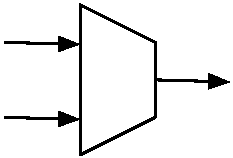
\includegraphics[scale=\scale]{../figures/mux}
\end{figure}
\shortlist{../code/mux.txt}
\begin{itemize}
\item So what?
\item Wait... What type is \code{a} and \code{b}?
\begin{itemize}
\item Can be any Chisel type!
\end{itemize}
\end{itemize}
\end{frame}

\begin{frame}[fragile]{Chisel has a Multiplexer}
\begin{figure}
  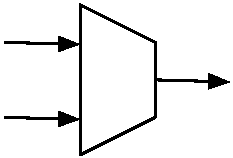
\includegraphics[scale=\scale]{../figures/mux}
\end{figure}
\shortlist{../code/mux.txt}
\begin{itemize}
\item SW people may not be impressed
\item They have generics since Java 1.5 in 2004
\begin{itemize}
\item \code{List<Flowers> != List<Cars>}
\end{itemize}
\end{itemize}
\end{frame}


\begin{frame}[fragile]{Generics in Hardware Construction}
\begin{itemize}
\item Chisel supports generic classes with type parameters
\item Write hardware generators independent of concrete type
\item This is a multiplexer \emph{generator}
\end{itemize}
\shortlist{../code/param_func.txt}
\end{frame}

\begin{frame}[fragile]{Put Generics Into Use}
\begin{itemize}
\item Let us implement a generic FIFO
\item Use the generic ready/valid interface from Chisel
\end{itemize}
\shortlist{../code/fifo_decoupled.txt}
\end{frame}

\begin{frame}[fragile]{Define the FIFO Interface}
\shortlist{../code/fifo_io.txt}
\begin{itemize}
\item We need enqueueing and dequeueing ports
\item Note the \code{Flipped}
\begin{itemize}
\item No more double definition of an interface
\end{itemize}
\end{itemize}
\end{frame}

\begin{frame}[fragile]{But What FIFO Implementation?}
\begin{itemize}
\item Bubble FIFO (good for low data rate)
\item Double buffer FIFO (fast restart)
\item FIFO with memory and pointers (for larger buffers)
\begin{itemize}
\item Using flip-flops
\item Using on-chip memory
\end{itemize}
\item And some more...
\end{itemize}
\begin{itemize}
\item This calls for object-oriented \sout{programming} \emph{hardware construction}
\end{itemize}
\end{frame}

\begin{frame}[fragile]{Abstract Base Class}
\shortlist{../code/fifo_abstract.txt}
\begin{itemize}
\item May contain common code
\item Extend by concrete classes
\end{itemize}
\begin{chisel}
class BubbleFifo[T <: Data](gen: T, depth: Int) extends Fifo(gen: T, depth: Int) {
\end{chisel}
\end{frame}



\begin{frame}[fragile]{Select a Concrete FIFO Implementation}
\begin{itemize}
\item Decide at hardware generation
\item Can use all Scala/Java power for the decision
\begin{itemize}
\item Connect to a web service, get \sout{Google} Alphabet stock price, and decide on which to use ;-)
\item For sure a silly idea, but you see what is possible...
\item Developers may find clever use of the Scala/Java power
\item We could present a GUI to the user to select from
\end{itemize}
\item We use XML files parsed at hardware generation time
\item End of TCL, Python,... generated hardware
\end{itemize}
\end{frame}

\begin{frame}[fragile]{Binary to BCD Conversion for VHDL}
\begin{figure}
    \centering
    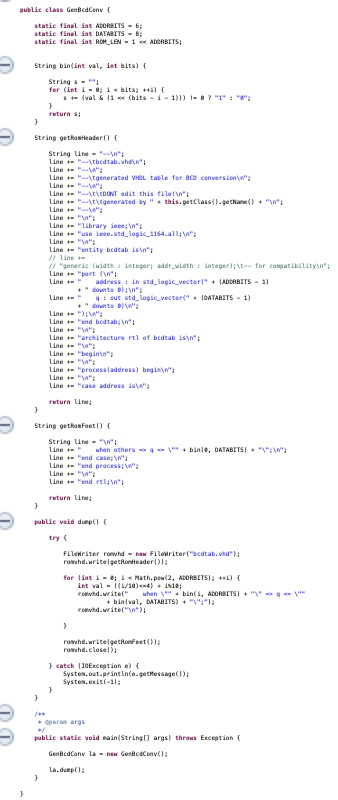
\includegraphics[scale=0.6]{JavaBCD}
\end{figure}
\end{frame}

\begin{frame}[fragile]{Java Program}
\begin{itemize}
\item Generates a VHDL table
\item The core code is:
\end{itemize}
\begin{chisel}
for (int i = 0; i < Math.pow(2, ADDRBITS); ++i) {
    int val = ((i/10)<<4) + i%10;
    // write out VHDL code for each line
\end{chisel}
\begin{itemize}
\item With all boilerplate 118 LoC
\end{itemize}
\end{frame}

\begin{frame}[fragile]{Chisel Version of Binary to BCD Conversion}
\begin{chisel}
  val array = new Array[Int](256)
  for (i <- 0 to 99) {
    array(i) = ((i/10)<<4) + i%10
  }
  val table = VecInit(array.map(_.U(8.W)))
\end{chisel}
\begin{itemize}
\item Directly generates the hardware (\code{VecInit})
\end{itemize}
\end{frame}

\begin{frame}[fragile]{Use Functional Programming for Generators}
\shortlist{../code/fun_first.txt}
\shortlist{../code/fun_func_lit.txt}
\shortlist{../code/fun_reduce_tree.txt}
\begin{itemize}
\item This is a simple example
\item What about an arbiter tree with fair arbitration?
\end{itemize}
\end{frame}

%\begin{frame}[fragile]{XXX}
%\begin{itemize}
%\item TODO: s4noc connection is part of the generator story
%\item
%\item
%\end{itemize}
%\end{frame}
%
%\begin{frame}[fragile]{XXX}
%\begin{itemize}
%\item
%\item
%\item
%\end{itemize}
%\end{frame}



\begin{frame}[fragile]{Generation Slides (include) are missing here}
\begin{itemize}
\item 
\end{itemize}
\end{frame}

\begin{frame}[fragile]{Combinational (Truth) Table Generation}
\begin{chisel}
val arr = new Array[Bits](length)
for (i <- 0 until length) {
  arr(i) = ...
}
val rom = Vec[Bits](arr)
\end{chisel}
\begin{itemize}
\item Generate a table in a Scala array
\item Use that array as input for a Chisel \code{Vec}
\item Generates a logic table at hardware construction time
\end{itemize}
\end{frame}

\begin{frame}[fragile]{BCD Generation Example}
\begin{itemize}
\item Explain BCD with examples
\item Show code
\end{itemize}
\end{frame}

\begin{frame}[fragile]{Ideas for Runtime Table Generation}
\begin{itemize}
\item Assembler in Scala/Java generates the boot ROM
\item Table with a \code{sin} function
\item Binary to BCD conversion
\item Schedule table for a TDM based network-on-chip
\item 
\item More ideas?
\end{itemize}
\end{frame}

\begin{frame}[fragile]{Memory}
\begin{chisel}
val mem = Mem(Bits(width = 8), size)

// write
when(wrEna) {
  mem(wrAddr) := wrData
}

// read
val rdAddrReg = Reg(next = rdAddr)
rdData := mem(rdAddrReg)
\end{chisel}
\begin{itemize}
\item Write is synchronous
\item Read can be asynchronous or synchronous
\item But there are no asynchronous memories in an FPGA
\end{itemize}
\end{frame}

\begin{frame}[fragile]{Factory Methods}
\begin{itemize}
\item Simpler component creation and use
\item Usage similar to built in components, such as \code{Mux}
\end{itemize}
\begin{chisel}
val myAdder = Adder(x, y)
\end{chisel}
\begin{itemize}
\item A little bit more work on component side
\item Define an \code{apply} method on the companion object that returns the component
\end{itemize}
\begin{chisel}
object Adder {
  def apply(a: UInt, b: UInt) = {
    val adder = Module(new Adder)
    adder.io.a := a
    adder.io.b := b
    adder.io.result
  }
}
\end{chisel}
\end{frame}

\begin{frame}[fragile]{Chisel and Scala}
\begin{itemize}
\item Chisel is a library written in Scala
\begin{itemize}
\item Import the library with \code{import chisel3.\_}
\end{itemize}
\item Chisel code is Scala code
\item When it is run is \emph{generates} hardware
\begin{itemize}
\item Verilog for synthesize
\item Scala netlist for simulation (testing)
\end{itemize}
\item Chisel is an embedded domain specific language
\item Two languages in one can be a little bit confusing
\end{itemize}
\end{frame}

\begin{frame}[fragile]{Scala}
\begin{itemize}
\item Is object oriented
\item Is functional
\item Strongly typed with very good type inference
\item Runs on the Java virtual machine
\item Can call Java libraries
\item Consider it as Java++
\begin{itemize}
\item Can almost be written like Java
\item With a more lightweight syntax
% \item Scala for Java Refugees is a nice tutorial (but link is dead)
% \item \url{http://www.codecommit.com/blog/scala/roundup-scala-for-java-refugees}
\end{itemize}
\end{itemize}
\end{frame}

\begin{frame}[fragile]{Scala Hello World}
\begin{chisel}
object HelloWorld extends App {
  println("Hello, World!")
}
\end{chisel}
\begin{itemize}
\item Compile with \code{scalac} and run with \code{scala}
\item You can even use Scala as scripting language
\item Show both
\end{itemize}
\end{frame}



\begin{frame}[fragile]{Generic Components}
\begin{chisel}
val c = Mux(cond, a, b)
\end{chisel}
\begin{itemize}
\item This is a multiplexer
\item Input can be any type
\end{itemize}
\end{frame}




\begin{frame}[fragile]{A Tiny ALU: IO Connection}
\begin{chisel}
class Alu extends Module {
  val io = IO(new Bundle {
    val fn = Input(UInt(2.W))
    val a = Input(UInt(4.W))
    val b = Input(UInt(4.W))
    val result = Output(UInt(4.W))
  })

  // Use shorter variable names
  val fn = io.fn
  val a = io.a
  val b = io.b
\end{chisel}
\end{frame}

\begin{frame}[fragile]{A Tiny ALU: The Function}
\begin{chisel}
  val result = Wire(UInt(4.W))
  // some default value is needed
  result := 0.U

  // The ALU selection
  switch(fn) {
    is(0.U) { result := a + b }
    is(1.U) { result := a - b }
    is(2.U) { result := a | b }
    is(3.U) { result := a & b }
  }

  // Output on the LEDs
  io.result := result
}
\end{chisel}
\end{frame}

\begin{frame}[fragile]{Testing the ALU}
\begin{itemize}
\item Compute the expected result in Scala
\end{itemize}
\begin{chisel}
  // This is exhaustive testing,
  // which usually is impossible
  for (a <- 0 to 15) {
    for (b <- 0 to 15) {
      for (op <- 0 to 3) {
        val result =
          op match {
            case 0 => a + b
            case 1 => a - b
            case 2 => a | b
            case 3 => a & b
          }
        val resMask = result & 0x0f
\end{chisel}

\end{frame}

\begin{frame}[fragile]{Testing the ALU}
\begin{itemize}
\item Compare the Scala computed result with the hardware result
\end{itemize}
\begin{chisel}
        poke(dut.io.fn, op)
        poke(dut.io.a, a)
        poke(dut.io.b, b)
        step(1)
        expect(dut.io.result, resMask)
      }
    }
  }
\end{chisel}
\end{frame}


\begin{frame}[fragile]{Summary}
\begin{itemize}
\item Chisel is a small language
\item Embedding it in Scala gives the power
\item We can write circuit generators
\item We can to co-simulation
\item We just scratched the surface
\end{itemize}
\end{frame}


\end{document}

%\begin{frame}[fragile]{xxx}
%\begin{itemize}
%\item yyy
%\end{itemize}
%\end{frame}
